\documentclass[12pt, spanish]{article}


\usepackage{scicite}

\usepackage{times}

\usepackage{graphicx}
\usepackage{caption}
\usepackage{subcaption}

\usepackage{hyperref}



\topmargin 0.0cm
\oddsidemargin 0.2cm
\textwidth 16cm 
\textheight 21cm
\footskip 1.0cm

\newenvironment{sciabstract}{%
\begin{quote} \bf}
{\end{quote}}

\renewcommand\refname{References and Notes}


\newcounter{lastnote}
\newenvironment{scilastnote}{%
\setcounter{lastnote}{\value{enumiv}}%
\addtocounter{lastnote}{+1}%
\begin{list}%
{\arabic{lastnote}.}
{\setlength{\leftmargin}{.22in}}
{\setlength{\labelsep}{.5em}}}
{\end{list}}


% Include your paper's title here

\title{Aprenentatge automàtic aplicat \\ al reconeixement de caràcters en imatges} 


% Place the author information here.  Please hand-code the contact
% information and notecalls; do *not* use \footnote commands.  Let the
% author contact information appear immediately below the author names
% as shown.  We would also prefer that you don't change the type-size
% settings shown here.

\author
{Francesc Aguirre,$^{1}$  Alberto Debernardi$^{2}$\\
\\
\normalsize{$^{1}$Autor: francesc.aguirre@gmail.com}\\
\normalsize{$^{2}$Tutor: adebernardipinos@gmail.com}\\
}

% Include the date command, but leave its argument blank.

\date{23/07/2021}


\begin{document} 
\pagenumbering{gobble}

% Double-space the manuscript.
\baselineskip24pt

\maketitle 

\baselineskip24pt

\begin{center}
	\includegraphics[width=0.15\textwidth]{images/Logo_uab}\par\vspace{1cm}
\end{center}

\clearpage


% Place your abstract within the special {sciabstract} environment.

\begin{sciabstract}
  Aquí anirà el resum en cat, cast, ang.
\end{sciabstract}

\clearpage

\tableofcontents

\clearpage

\pagenumbering{arabic}
%%% (1)
\section{Introducció}

L'estadística és la disciplina que s'encarrega d'analitzar dades per a respondre a preguntes empíriques. A mitjans del segle XX, amb la creació dels dispositius electrònics d'emmagatzematge i l'ajuda de sensors, la quantitat d'informació que es pot recol·lectar ha crescut any rere any. Aquest fet ha donat lloc al naixement de noves disciplines d'anàlisi de dades, tals com la mineria de dades i l'aprenentatge automàtic, més conegut pel seu nom en anglès \textit{machine learning}.

El machine learning és un conjunt de tècniques que dóna als ordinadors l'habilitat d'aprendre de les dades. S'utilitza per a resoldre una gran varietat de problemes predictius complexos en els àmbits d'economia i finances, bioinformàtica, salut, meteorologia, màrqueting, problemes en l'anàlisi i classificació d'imatges, vídeos, àudio... En l'àmbit de l'anàlisi d'imatges hi ha la detecció d'objectes, i més concretament, el reconeixement òptic de caràcters. 

En aquest estudi s'investigarà l'àmbit del reconeixement òptic de caràcters, i com obtenir models predictius competents utilitzant tècniques de machine learning. Per a posar aquests coneixements en pràctica, es resoldrà un problema d'identificació de caràcters irregulars en imatges, tal com la identificació d'escriptura manual o la resolució de \textit{captcha} (és a dir, text en una determinada font que inclou una certa distorsió, precisament per evitar la detecció dels caràcters per part de models més simples, i que són àmpliament utilitzats en internet per evitar l'automatització de determinats processos).


%%% (2)
\section{OCR}

El reconeixement òptic de caràcters OCR (de les sigles en anglès \textit{Optical Character Recognition}) és una aplicació de la intel·ligència artificial, que té com a objectiu detectar i identificar els caràcters que es puguin trobar en una imatge. És una de les àrees més estudiades en l'àmbit de reconeixement de patrons gràcies al gran nombre d'aplicacions pràctiques. Alguns dels problemes que OCR pot ajudar a agilitzar i automatitzar són la digitalització de diaris i llibres antics, la identificació de matrícules, la classificació d'imatges segons el text detectat, i la lectura de dades en paper tals com documentació, correu i enquestes. La digitalització a ordinador de text té moltes més aplicacions, tals com la cerca, edició i emmagatzematge d'informació, traducció, transcripció de text a àudio i NLP (de les sigles en angles \textit{Natural Language Processing}).


% (2.1)
\subsection{Parts tradicionals d'un sistema OCR}

Tradicionalment, un problema típic d'OCR es pot dividir en subtasques en forma de \textit{pipeline} (fetes una darrera l'altre en un ordre concret) que utilitzen tècniques de visió artificial (en anglès \textit{computer vision}), estadístiques i de machine learning. És útil conèixer-les per saber en quin punt del sistema s'està \cite{chaudhuri2017optical}.

\begin{enumerate}
\item Escaneig: És el procés d'escanejar o fotografiar el text \textit{input}. Normalment, al d'escanejar un document s'aplica \textit{thresholding} (binarització) per estalviar memòria i capacitat computacional, que és una tècnica que dicotomitza el color gris de documents en blanc i negre segons un llindar d'intensitat.

\item Segmentació de text: Un cop escanejat el document, típicament el que es vol és obtenir un sol caràcter per utilitzar-lo d'input en el model. La segmentació d'una imatge és la divisió d'aquesta en parts. En aquesta tasca, el que es vol és localitzar el text que ens interessa i ometre gràfics, imatges, logotips... Tot seguit es vol segmentar línies de text, de les línies es segmenten paraules, i de les paraules se segmenten caràcters. En la segmentació ens podem trobar diversos problemes, sobretot si un caràcter està format per diferents parts (i j), si s'està tocant amb algun altre, o s'ha dividit.

\item Preprocessament: Com que el fet d'escanejar o fotografiar una imatge és un procés variable (brillantor, angle...), els caràcters de la imatge segmentada poden contenir soroll, o estar trencats. El preprocessament té com a objectiu eliminar soroll, omplir espais trencats i reduir la grossor dels píxels negres que formen el caràcter. També es normalitzen les dimensions i s'aplicarà una rotació si es detecta inclinació.

\item Segmentació interna: Consisteix a segmentar la imatge del caràcter en seccions més petites, tals com línies i corbes concretes. La intensió és començar a detectar zones amb patrons concrets que facilitin el reconeixement posterior del caràcter.

\item Extracció de variables: A partir de la segmentació interna, se seleccionarà un conjunt de variables que maximitzi el reconeixement amb el nombre menor d'elements. L'objectiu és capturar característiques essencials dels símbols per posteriorment entrenar el model. La extracció de variables més sencilla sería utilitzar la matriu de pixels de la imatge, tot i que utilitzar tantes variables pot provocar problemes de dimensionalitat en molts dels models. Utilitzant extracció de variables, s'utilitzarien característiques que descriguin els caràcters, tals com llargades de segments en regions de la imatge, angles de curvatura...

\item Entrenament i reconeixement: Aplicació de tècniques de reconeixement de patrons per a classificar el caràcter. Aquí és on podem utilitzar tècniques estadístiques i de machine learning per fer la classificació, tals com (TODO)...

\item Reagrupació de caràcters a paraules, paraules a línies, fins a tenir el document complet.
\end{enumerate}

Com es pot veure, la creació d'un sistema OCR tradicional és un procés llarg, amb moltes subtasques que relativament complicades. Els avantatges dels mètodes tradicionals és que donen bons resultats amb mostres petites i són computacionalment eficients. Alguns dels inconvenients és que utilitzen detecció i segmentació de text a partir de tècniques de visió artificial no relacionades amb machine learning, és a dir, no aprenen de les dades. Com que la segmentació no sempre és evident, i les dades poden ser sorolloses, utilitzar aquest tipus de tècniques acostuma a produir errors difícils de solucionar.


% (2.2)
\subsection{Sistema OCR a l'actualitat}

Aquests últims anys, a partir del 2010, el desenvolupament de la branca \textit{deep learning} (aprenentatge profund, una branca de machine learning) a tingut un avanç molt important. La solució en les xarxes neuronals del problema de \textit{vanishing/exploding gradients} i el llançament de noves tecnologies d'alta capacitat computacional tals com noves GPU (de les sigles en anglès \textit{graphics processing unit}), a permès l'entrenament de xarxes neuronals profundes (DNN de les sigles en anglès \textit{deep neural networks}).

Aquest desenvolupament ha donat lloc a nous sistemes OCR basats en xarxes neuronals. La majoria del preprocessament i binarització no és necessari, ja que les xarxes neuronals s'adapten als inputs, podent utilitzar fàcilment els píxels de les imatges. La segmentació de text es pot fer amb tècniques basades en DNN tals com FCN (de les sigles en anglès \textit{Fully Convolutional Networks}), donant millors resultats que amb les tècniques de visió artificial. A més a més, si s'utilitzen RNN (de les sigles en anglès \textit{Recurrent Neural Networks}), no cal segmentar caràcter a caràcter, sinó que es poden utilitzar línies completes de text. Un altre avantatge de les RNN és que poden aprendre de manera natural la llengua utilitzada en l'entrenament. La tendència actual és utilitzar FCN per la segmentació de text en línies, i utilitzar RNN pel seu reconeixement, juntament amb CNN (de les sigles en anglès \textit{Convolutional Neural Networks}) per fer l'extracció de variables \cite{martinek2020building}.

\clearpage
%%% (3)
\section{Problema pràctic}

En aquesta secció es buscaran solucions a un problema pràctic d'OCR. L'objectiu és introduir recursos que ajudin a solucionar un problema del reconeixement de caràcters, i veure quina solució dóna millors resultats. 

Inicialment es buscarà solucionar un problema de reconeixement de caràcters escrits a mà. A primera vista aquest no és un problema fàcil. Hi ha 62 caràcters diferents en l'alfabet anglès, el que implica que a partir d'una imatge, l'algoritme haurà de seleccionar un caràcter entre els 62 disponibles (classes). Si es volgués utilitzar el nostre model per automatitzar completament un procés, es buscaria una precisió propera al 99.5\%. Si es té algú vigilant l'algoritme, llegint que el reconeixement tingui sentit, es pot demanar una precisió més baixa, entre 95\% i 99\%. A més a més, si el que s'analitza són caràcters individuals (sistema tradicional, part de segmentació de text), normalment aquest caràcter forma part d'una paraula, i si aquesta paraula no existeix en el vocabulari, podem fer que el sistema ens avisi (o per exemple, si volem llegir els NIU o id d'alumnes, podem detectar si existeix el NIU reconegut). Per tant, tot i no aconseguir la precisió més alta, el sistema pot seguir sent útil i no fer errors tan fàcilment. 

% (3.1)
\subsection{Base de dades}

Per a l'elecció de la base de dades, com que s'està experimentant i no es té un objectiu estricte (no s'està participant o ajudant en cap projecte extern al treball), s'ha optat per una base de dades amb una bona quantitat d'exemples i dades ja preprocessades, ja que el preprocessament de dades és una part molt tècnica i metòdica. S'han trobat diferents opcions gratuïtes disponibles en internet, i finalment s'ha utilitzat la base de dades d'imatges de caràcters EMNIST \cite{EMNIST}, derivada de la base de dades d'OCR NIST \cite{watson1992nist}.

La base de dades NIST consisteix en 3669 imatges binaritzades de mostres de formularis fets expressament per testejar mètodes de reconeixement de caràcters (fig:\ref{fig:nist1}). La base de dades també conté els 814,255 caràcters resultants d'aplicar segmentació de text sobre el formulari, en forma d'imatges png de dimensions 128x128 píxels, etiquetades de "0" - "9", de "A" - "Z" i de "a" - "z" en notació hexadecimal. Les imatges segmentades s'han ordenat i etiquetat en diferents organitzacions de carpetes:

\begin{figure}
\centering
\begin{minipage}{.5\textwidth}
  \centering
  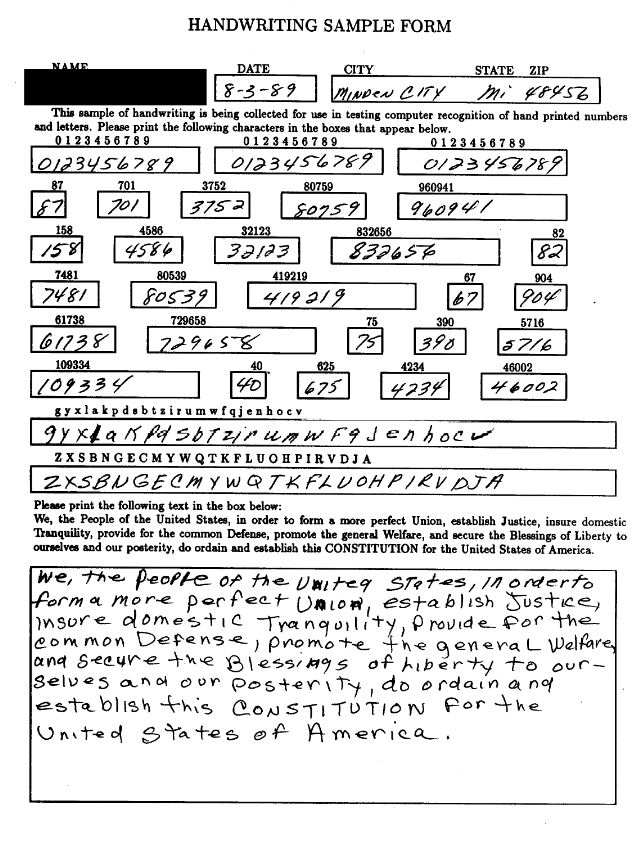
\includegraphics[width=1\linewidth]{images/nist1.jpg}
  \captionof{figure}{Exemple formulari NIST \cite{watson1992nist}}
  \label{fig:nist1}
\end{minipage}%
\begin{minipage}{.5\textwidth}
  \centering
  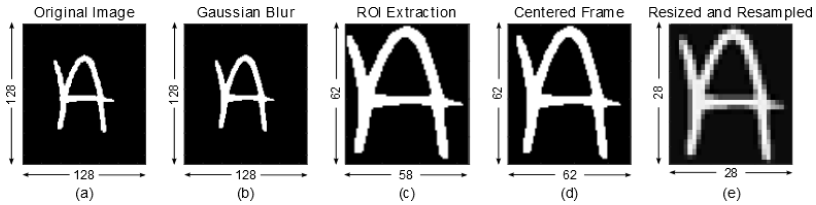
\includegraphics[width=1\linewidth]{images/emnist1.png}
  \captionof{figure}{Transformació d'una imatge NIST a EMNIST \cite{EMNIST}}
  \label{fig:emnist1}
\end{minipage}
\end{figure}

\begin{itemize}
\item Per autor: Els 3669 formularis s'han omplert per persones diferents. Els caràcters segmentats resultants de cada formular-hi s'han agrupat per persona. Aquesta organització no és útil per OCR, sinó per diferenciar tipus d'escriptura segons individus.

\item Per tipus de camp: Les imatges de caràcters s'han dividit pels diferents blocs del formulari: dígits, minúscules, majúscules i text. Seguidament s'han separat per classe de caràcter. Aquest tipus d'organització pot ser molt útil si volem fer models que només continguin un tipus de camp. Per exemple, hi ha tasques, tals com reconeixement de caràcters de formularis, on es demana que s'escrigui només en majúscules, o potser només es volen reconèixer dígits. Entrenar un model amb un nombre de classes possibles reduït serà molt més fàcil que entrenar un model amb 62 classes. A més a més, hi ha classes de caràcters similars de camps diferents ("0", "o", "O"; "I", "l", "1"), que al redimensionar les dimensions de la imatge costaran molt d'identificar. Els diferents camps són fàcils d'identificar en una frase o paraula (majúscules només a l'inici de noms personals o frases, no barrejar números i lletres en una paraula...), però si es barregen les 62 classes a la vegada i s'intenten reconèixer, la dificultat del problema augmentarà, cosa que s'ha de tenir en compte. Aquest també és un dels motius per al que l'ús de RNN per analitzar línies senceres de text funcionen molt bé, perquè aprenen el llenguatge de manera natural, resolent automàticament el problema dels diferents tipus de camps. 

\item Per classe: Les imatges de caràcters estan agrupats en les 62 carpetes de les diferents classes. Amb aquesta organització, tenim el problema de no poder diferenciar entre tipus de camps. 

\item Per classes unides: Com que amb l'organització per classe hi ha classes massa similars entre elles, s'ha creat una nova organització ajuntant les classes entre minúscules i majúscules  que s'han considerat més similars (C, I, J, K, L, M, O, P, S, U, V, W, X, Y, Z), fent un total de 47 classes diferents.




\end{itemize}









% Fitxer bibliografia scibib.bib

\clearpage
\bibliography{scibib}

\bibliographystyle{Science}


% Citacions extra manuals

\begin{scilastnote}
\item Codi desenvolupat: \href{https://github.com/cesc1/TFG}{github/cesc1/TFG}

\end{scilastnote}


\end{document}




















